\section{Three-dimensional domains}
\label{sec_domains}

As stated before, {\psiboil} supports three-dimensional Cartesian
computational domains, defined by objects of type {\tt Domain}. 
It uses three one-dimensional grids {\tt Grid1D} to define 
resolution in each of the coordinate direction ($x$, $y$ and $z$).

The following program ({\tt 05-04-main.cpp}) creates a cubical domain, 
having dimension $1 \times 1 \times 1$, with uniform cell distribution 
in $x$ and $y$ direction, while stretched towards both ends in $z$ 
direction: 
%
{\small \begin{verbatim}
      1 #include "Include/psi-boil.h"
      2
      3 const real L = 3.2;
      4 const real D = 0.01;
      5 const int  N = 32;
      6
      7 /****************************************************************************/
      8 main(int argc, char * argv[]) {
      9
     10   boil::timer.start();
     11
     12   /* uniform grid */
     13   Grid1D g_uni( Range<real>(-0.5*L, 0.5*L), N, Periodic::no() );
     14
     15   /* stretched grid */
     16   Grid1D g_str( Range<real>(0,L), Range<real>(D,D), N*2, Periodic::no());
     17
     18   /* create domain */
     19   Domain dom(g_uni, g_uni, g_str);
     20
     21   /* plot the domain */
     22   boil::plot = new PlotTEC();
     23   boil::plot->plot(dom, "dom");
     24
     25   boil::timer.stop();
     26   boil::timer.report();
     27 }
\end{verbatim}}
%
Line~13 creates {\tt g\_uni}, a uniform grid with~32 cells, ranging 
from~$\xi=-1.6$ to $\xi=1.6$. Line~16 creates {\tt g\_str}, a grid ranging from 
$\xi=0$ to $\xi=3.2$ which is stretched towards both ends. Note that the size of
cells next to the boundaries of {\tt g\_str} is~$\Delta \xi = 0.01$. 

Command which creates the computational domain is in line~19. This line creates
an object of type~{\tt Domain}, called~{\tt dom}. It's constructor accepts three
arguments: grid in $x$, $y$ and $z$ direction. In this particular case, we use
grid~{\tt g\_uni} for distribution in $x$ and $y$, and grid~{\tt g\_str} to
define distribution in~$z$ direction.

Domain is plotted in lines~21--23. Plotting is performed with the global {\psiboil}
object~{\tt boil::plot}. This global object can be created in two ways, depending
on the format of output files you would like to create. If you would like to plot
your grids (and later results) in Tecplot\footnote{Tecplot is a registered trademark
of Tecplot Inc.\ ({\tt www.tecplot.com})} format,
create the {\tt boil::plot} as in line~22. If you prefer output files in General
Mesh Viewer\footnote{{\tt www-xdiv.lanl.gov/XCM/gmv/GMVHome.html}}~(GMV) format, 
change the line~22 to:
%
{\small \begin{verbatim}
     22   boil::plot = new PlotGMV();
\end{verbatim}}
%
When running the program~{\tt 05-04-main.cpp}, you will get the following output:
%
{\small \begin{verbatim}
Domain level 4 created !
Domain level 3 created !
Domain level 2 created !
Domain level 1 created !
# Plotting: dom_p000.dat
+==========================================
| Total execution time: 0.18 [s]
+------------------------------------------
| Time spent in plotting: 0.18 [s]    (100%)
| Time spent elsewhere: 0 [s]    (0%)
+------------------------------------------
\end{verbatim}}
%
The output informs you that it has created four grid levels in addition to the
one specified by the user. The level specified by the user is always level~0,
while the coarser levels have larger numbers. Thus, for this particular case,
level~0 will have resolution of:~$32 \times 32 \times 64$, 
level~1: $16 \times 16 \times 32$, level~2: $8 \times 8 \times 16$, 
level~3: $4 \times 4 \times 8$ and, finally, level~4 will have the coarsest 
resolution of only $4 \times 4 \times 4$ cells. 

The grid on the finest level (level~0) is plotted from line~23, using the global
object~{\tt boil::plot} and its member function {\tt boil::plot->plot()}. As the
arguments, you send the {\tt Domain} to be plotted (in this case it is {\tt dom})
and the name you want to associate with it ({\tt "dom"}). The plotting function
({\tt boil::plot->plot()}) names the output file as: {\tt dom\_p000.dat}, where
{\tt \_p000} is processor number and {\tt .dat} is extension recognized by
Tecplot. The grid on the finest level, visualized by Tecplot is shown in 
Fig.~\ref{fig_domain_l0}. 

In case that you executed ./Boil using multiple processes, e.g. 
{\tt> mpirun -np 4 ./Boil}, it is inconvenient to have multiple dat-files for the 
visualization. In order to create single dat-file from multiple-files, an utility 
program can be used.
%
{\small \begin{verbatim}
> cd ~/Development/PSI-Boil/Src/Utility/Gather
> ifort -fpp -DVISIT gather.f90 ./tecio64.a -lm -lstdc++ -o gather.exe
> ifort -fpp -DVISIT -DZIP gather.f90 ./tecio64.a -lm -lstdc++ -o gather-zip.exe
\end{verbatim}}
%
Copy {\tt gather.exe} and {\tt gather-zip.exe} in {\tt Src} directory or the directory
where the path is set. {\tt gather.exe} read the dat-files, and exports a plt-file.
Here plt-file is the binary format data file for Tecplot. In case of {\tt gather-zip.exe},
the output file is zipped plt-file. Please note that the data of an immersed body 
disappears during this file-format conversion.

The open-source visualization software VisIt\footnote{https://visit-dav.github.io/visit-website/} 
can import plt-file, and draw a similar picture as Fig.~\ref{fig_domain_l0}.
Note that VisIt cannot import dat-file, which is output from {\tt psi-boil}.

%----------%
%          %
%  Domain  %
%          %
%----------%
\begin{figure}[ht]
  \centering
  \setlength{\unitlength}{1mm}
  \begin{picture}(80,65)(0,0)
    \thickbox{80}{65}
    \put(0,0){\includegraphics[scale=0.33]{Figures/05-04-domain-l0.eps}}
  \end{picture}
  \caption{Stretched computational domain.}
  \label{fig_domain_l0}
\end{figure}

Note that program reports on the time spent in plotting functions with:
%
{\small \begin{verbatim}
| Time spent in plotting: 0.18 [s]    (100%)
\end{verbatim}}
%
That is because all the plotting functions are embedded in {\em local} 
timing routines, such as the ones introduced in the section~\ref{sec_local}.

You have to stretch the grid towards the walls very often, but sometimes
you might also want to stretch in the interior - particuluarly if there
are obstacles (or inner walls) inside. A way to achieve such a stretching
is to combine two stretched grids together. The way to do it is demostrated
below. The lines of the {\tt 05-04-main.cpp} code are replaced with the 
following (to get the program {\tt 05-05-main.cpp}):
%
{\small \begin{verbatim}
     15   /* stretched grid */
     16   Grid1D g_str( Range<real>(0,0.5*L), Range<real>(D,D), N, Periodic::no());
     17
     18   Grid1D g_str_2(g_str, g_str, Periodic::no());
     19
     20   /* create domain */
     21   Domain dom(g_uni, g_uni, g_str_2);
\end{verbatim}}
%
{\tt Grid1D g\_str} is still created in line~16, but this time is half
as short and it has half as many cells as in the previous case. Next,
additional grid is created in line~18, where two {\tt g\_str}'s are
added one after another. The {\tt Grid1D} constructor in line~18 
takes two {\tt Grid1D}'s as parameters, leaves the absolute coordinates
of the first intact, but disregards the absolute coordinates of the second.
It shifts and attaches the grid sent as second parameter to the grid sent
as first parameter\footnote{If it was not shifting the second, they
would collapse into one grid for this case.}. 
Finally, {\tt Domain dom} is created in line~21 using the new,
double-stretched grid to set the resolution in~$z$ direction, and
is plotted in~Fig.~\ref{fig_domain_double_stretched}. 

%
%----------------------------%
%                            %
%  Domain - duble stretched  %
%                            %
%----------------------------%
\begin{figure}[ht]
  \centering
  \setlength{\unitlength}{1mm}
  \begin{picture}(80,65)(0,0)
    \thickbox{80}{65}
    \put(0,0){\includegraphics[scale=0.33]{Figures/05-04-double-stretch.eps}}
  \end{picture}
  \caption{Double-stretched computational domain.}
  \label{fig_domain_double_stretched}
\end{figure}

% remove? \subsection{Implicit plotting}
% remove? 
% remove? In the program example {\tt 05-04-main.cpp} you have explicitly 
% remove? plotted the computational domain from lines~21--23. This plotted only
% remove? the finest grid level. There is a way to plot coarser grid levels as
% remove? well. To achieve that, remove lines 21 and 22 from~{\tt 05-04-main.cpp}
% remove? and move the line~23 above the definition of the {\tt Domain dom}.
% remove? You might even place it just after starting the timer (line~10), to 
% remove? get the listing ({\tt 05-05-main.cpp}):
% remove? %
% remove? {\small \begin{verbatim}
% remove?       1 #include "Include/psi-boil.h"
% remove?       2
% remove?       3 const real L = 3.2;
% remove?       4 const real D = 0.01;
% remove?       5 const int  N = 32;
% remove?       6
% remove?       7 /****************************************************************************/
% remove?       8 main(int argc, char * argv[]) {
% remove?       9
% remove?      10   boil::timer.start();
% remove?      11
% remove?      12   /* plot in Tecplot format */
% remove?      13   boil::plot = new PlotTEC();
% remove?      14
% remove?      15   /* uniform grid */
% remove?      16   Grid1D g_uni( Range<real>(-0.5*L, 0.5*L), N, Periodic::no() );
% remove?      17
% remove?      18   /* stretched grid */
% remove?      19   Grid1D g_str( Range<real>(0,L), Range<real>(D,D), N*2, Periodic::no());
% remove?      20
% remove?      21   /* create domain */
% remove?      22   Domain dom(g_uni, g_uni, g_str);
% remove?      23
% remove?      24   boil::timer.stop();
% remove?      25   boil::timer.report();
% remove?      26 }
% remove? \end{verbatim}}
% remove? %
% remove? When compiled and ran, this program creates the output:
% remove? %
% remove? {\small \begin{verbatim}
% remove? Domain level 4 created !
% remove? # Plotting: domain_p000_0004.dat
% remove? Domain level 3 created !
% remove? # Plotting: domain_p000_0003.dat
% remove? Domain level 2 created !
% remove? # Plotting: domain_p000_0002.dat
% remove? Domain level 1 created !
% remove? # Plotting: domain_p000_0001.dat
% remove? # Plotting: domain_p000_0000.dat
% remove? +==========================================
% remove? | Total execution time: 0.22 [s]
% remove? +------------------------------------------
% remove? | Time spent in plotting: 0.22 [s]    (100%)
% remove? | Time spent elsewhere: 0 [s]    (0%)
% remove? +------------------------------------------
% remove? \end{verbatim}}
% remove? %
% remove? This time it plotted each domain level it created, from finest level, stored
% remove? in file {\tt domain\_p000\_0000.dat}, to the coarsest one stored in
% remove? {\tt domain\_p000\_0004.dat}. The four-digit number before the file extension
% remove? denotes the grid level. 
% remove? For example, level~2 is shown in Fig.~\ref{fig_domain_l2}.
% remove? 
% remove? %----------%
% remove? %          %
% remove? %  Domain  %
% remove? %          %
% remove? %----------%
% remove? \begin{figure}[ht]
% remove?   \centering
% remove?   \setlength{\unitlength}{1mm}
% remove?   \begin{picture}(80,65)(0,0)
% remove?     \thickbox{80}{65}
% remove?     \put(0,0){\includegraphics[scale=0.33]{Figures/05-05-domain-l2.eps}}
% remove?   \end{picture}
% remove?   \caption{Computational domain at level 2, visualized with Tecplot.}
% remove?   \label{fig_domain_l2}
% remove? \end{figure}
% remove? 
% remove? This {\em implicit} plotting was introduced in early stages of {\psiboil} 
% remove? development, when the main concern was the multigrid solver. If it annoys you,
% remove? simply define {\tt boil::plot} after the definition of a {\tt Domain} and
% remove? {\psiboil} will not do it. 

%---------------------------------------------------------------------nutshell-%
\vspace*{5mm} \fbox{ \begin{minipage}[c] {0.97\textwidth} %-----------nutshell-%
    {\sf Section \ref{sec_domains} in a nutshell} \\  %---------------nutshell-%
   
      - Three-dimensional Cartesian grids, represent with class {\tt Domain}, 
      are created from three one-dimensional grids ({\tt Grid1D}), with 
      the constructor:
      \begin{itemize}
        \item {\tt Domain(Grid1D \& gx, Grid1D \& gy, Grid1D \& gz);}
      \end{itemize}
      where {\tt gx}, {\tt gy} and {\tt gz} represent grid resolutions
      in $x$, $y$ and $z$ coordinate directions. \\
  
      - In order to plot domains, global object {\tt boil::plot} must be 
      defined before it is used. \\
 
      - {\tt boil::plot} can be defined as:
      \begin{itemize}
        \item {\tt boil::plot = new PlotGMV();} for plotting with GMV,
        \item {\tt boil::plot = new PlotTEC();} for plotting with Tecplot.
      \end{itemize}

      - Grids ({\tt Grid1D}) can also be constructed by appending one
      after another, using the constructor: 
      {\tt Grid1D(Grid1D \&, Grid1D \&, Periodic)}. \\

      - {\tt Domain}s can be plotted explicitly, using the command:
      \begin{itemize}
        \item {\tt boil::plot->plot(Domain \& dom, "file\_name");}
      \end{itemize}
% remove?       or implicitly, just by defining {\tt boil::plot} before the
% remove?       {\tt Domain}.
    
  \end{minipage} } %--------------------------------------------------nutshell-%
%---------------------------------------------------------------------nutshell-%
